%
% File acl2015.tex
%%
%% Based on the style files for ACL-2014, which were, in turn,

%% and that of ACL 08 by Joakim Nivre and Noah Smith

\documentclass[11pt]{article}
\usepackage{acl2015}
\usepackage{times}
\usepackage{url}
\usepackage{latexsym}
\usepackage[colorlinks,linkcolor=blue]{hyperref}
\usepackage{float}
\usepackage{graphicx}
\graphicspath{ {./images/} }
% \usepackage{cite}

% \setlength\titlebox{5cm}

% You can expand the titlebox if you need extra space
% to show all the authors. Please do not make the titlebox
% smaller than 5cm (the original size); we will check this
% in the camera-ready version and ask you to change it back.


\title{Text mining on Novels}

\author{Xiangyu Wei \\
  CIMS \\
  New York University \\
  {\tt xw1882@nyu.edu} \\\And
  Yunhao Li \\ 
  CIMS \\
  New York University \\
  {\tt yl6220@nyu.edu} \\\And
  Kaili Ding \\ 
  CIMS \\
  New York University \\
  {\tt kd2164@nyu.edu} \\}

% \date{}

\begin{document}
\maketitle
\begin{abstract} % Yunhao Li
  We develop a system that can automatically mining the data of novels. The system includes name entity recognition and merging, coreference resolution, interaction and sentiment analysis and relation extraction. Finally, we test it on two novels and visualize the result, which shows that our system runs well.
\end{abstract}

\section{Introduction} % Yunhao Li

The information extraction is an interesting field in Natural Language Processing(NLP). And text mining is an information extraction process for deriving high-quality information from text. As one of the most popular genres of literature, novel always have a lot of information between roles. Remembering all the roles and their relationships is somewhat hard for readers. A system that can help the readers understand the novel will be great. \\

In this paper we aims at mining the sentiment and social relationships between roles of the novels. To detect all the roles showing up in the novel, we need to do name entity recognition. Considering that every roles may have several names in one novel(e.g. Ronald Weasley, aka Ron, Ron Weasley, Mr.Weasley), we need to find a way to merge these alias and point them to the correlated role. This part will be introduced in part 3.1. \\

Coreference resolution is also essential. A role in the novel may always occur with a pronoun instead of his/her real name (or alias). If we just do the search with their names, we are not able to find enough information. Part 3.2 will explain how we do coreference resolution in detail.  \\

Part 3.3 introduces the text processing to get a sentences list where all pronoun replaced by the most possible correlated name, which will be replaced by its formatted name later.  \\

Having the pre-processed sentences list, we will do interaction and sentiment analysis. We get a interact matrix by analyzing each sentence. And we use two different methods to get the sentiment polarity scores of the sentence. We also build the sentiment matrices to do some analysis, including clustering analysis(using scikit-learn~\cite{sklearn_api}. Part 3.4 will provide the explanation. \\

In relation extraction part, we implement a method combining the algorithms introduced by Kokkinakis~\cite{kokkinakis-malm-2011-character} and Makazhanov ~\cite{Makazhanov2014ExtractingFR}. It works very well on the novels. We can extract a clear social relation(parent, children, siblings, etc). And we visualize the results. The details are in part 3.5 and Experiments. \\

We do the tests on two novels, \textit{Harry Potter and the Sorcerer's Stone}~\cite{harrypotter} and \textit{Pride and Prejudice}~\cite{pride}. The details of the results are shown in Experiment part.

% cite
\section{Related work} % Yunhao Li
Text mining on novels is an integral project instead of a single target. So we search the related work in different fields of NLP.\\

In the name entity recognition(NER), there is lots of libraries provide NER API for developers to use, such as CoreNLP~\cite{corenlp}, NLTK~\cite{Loper02nltk:the}, Spacy~\cite{honnibal-johnson:2015:EMNLP}, etc. They provide a good result of NER.\\

For the sentiment analysis, there is a lot of libraries and APIs provided by research institute or companies. Companies like Facebook, Google, Baidu, Tencent, etc, provide API 
for sentiment analysis. However, the Google's API is not free, which means unusable for us. The APIs of Baidu and Tencent only work well on Chinese texts. When testing on English text it doesn't perform well. We finally find nltk.sentiment.vader~\cite{Vader} works well on sentiment analysis. \\

Coreference resolution is an important field in NLP. The models of Clark and Manning~\cite{clark-manning-2016-deep}, based on Deep Learning, works well in our project. \\

We also find several papers works well in relation extraction. For extacting the family relation and social relation, Makazhanov's work~\cite{Makazhanov2014ExtractingFR} gives us a good point. And Kokkinakis and Malm~\cite{kokkinakis-malm-2011-character} also shows a way to extract relationship in Novel.


\section{Approaches}
It is a integral system that works on processing the novel in our work. It can be split into several parts introduced in the following sections.

\subsection{Role entity recognition and merging} % Kaili Ding

The very first step of the whole pipeline is to extract names of roles in the novel and merge the alias of one role as accurate as possible so that we can prevent multiple roles presenting one role in our final results. The merging step can make our results more accurate. \\

To extract names, we use name entity extractor in StanfordNLP library~\cite{stanfordnlp}, which tags names with ``PERSON" tag. We run the extractor on the novels, and consider continuous words tagged with ``PERSON" as a name. For the novel Harry Potter, after the raw extraction, we have 228 names. \\

Clearly, there are too many names for us to generate a clear relationship among roles. Therefore, we decide to reduce names we have extracted. By manually looking into the names we extracted, we find that for some roles, there are many alias for them. Essentially, these alias can be classified into three types. The first type is alias from typo. For example, we have ``Quirrell" and ``Quirtell", which are obviously aliases of the same entity. The second type is alias of part of names. For example, we have both ``Harry" and ``Harry Potter" in our novel. In this case, we need find a way to merge them, otherwise, we will have both ``Harry" and ``Harry Potter" in our final results as noise. The final type is alias of nicknames of the same entity, such as ``Nicolas" and ``Nick", and ``Johnson" and ``Johnny". \\

To deal with the typo alias, we can take advantage of the characteristics that the typo is only about one or at most two characters in a word, and most of the characters and their order are correct even there is a typo. We need to introduce a measure of similarity between words. We used both Soundex system and Jaro distance. The Soundex system~\cite{Soundex} is to assign a code to a word based on a set of pronunciation rule. The code consist of a letter, which is the first letter of the word, and three digits. The basic idea behind this system is we ignore vowel characters and group some consonant characters that have similar pronunciation and assign them a single digit. We stop once we get three digits on this word, or append 0 if the word cannot generate three digits. In our case, we regard two words as the same if they have the same Soundex code. The Jaro distance~\cite{Jaro} is a measure on the strings themselves. Basically, we calculate the number of matching characters in two words, and then further the proportion of matching characters in both strings. The order of matching characters should be the same, but we allow some transposition of characters whose distance is smaller than certain value in original words. The measure will generate a value between 0 and 1, and the larger the value is, the more similar the two words are. Applying both methods, we find that although Soundex system provides fewer aliases (merges more aliases), it mistakenly merges some aliases. Thus, we decide to use Jaro distance to merge aliases at last. \\

To tackle aliases from part of names, we split two names by space and check whether one name contain the other. The contain here is defined as one name has all the same words in the other name in the same order. Considering the existence of typo, we use Jaro distance again when we compare two words. If one name is contained by only one other name, then we merge the contained name into the name contains it. \\

For the alias of nickname, we haven't find a good way to merge them, since their pronunciation is different and similarity is low. One possible way to deal with this situation is have a dictionary of original name and nickname. However, the drawback of this solution is that the relationship among original name and nickname may not be one to one. \\

Furthermore, we add other features on extraction. We keep the prefix (Mr. and Mrs.) when extracting names as an indication of the gender. There are many roles who just appear several times in a novel, and we decide to drop them by setting a threshold to make the relationship map clearer. We also distinguish the family names and prevent merging them into other names. If we don't apply this rule, ``Weasleys" will be merged into ``Ron Weasley", which is not accurate. Finally, we assign a formatted name to each group after we do the merge. We will replace aliases and pronouns in the novel with the formatted names later.

\subsection{Coreference resolution} % Xiangyu Wei
\label{sect:pdf}

When the names of roles have been extracted, we need to find out in which scenarios these characters appear in the novel. Considering most of the characters are mentioned in a novel as pronouns like ``she", ``he" or ``they", it is important to match these pronouns with the names we have extracted. That is, we need do reference resolution for the text in the novel.

First, we tried the traditional rule-based method to do reference resolution for a text. We simply go through the text and do name-entity recognition using Spacy package in Python~\cite{honnibal-johnson:2015:EMNLP}. When meeting a pronoun whose reference is unknown, we just search in previous sentences and use the first entity labelled ``PERSON" which can match the pronoun in gender and number. To predict the gender of a given name, we used Clint Valentine's gender-predictor Python package~\cite{gender_predictor}. Considering we need to do a search for almost every pronouns like ``he", ``she" or ``they", the depth of each search can not be too large. Otherwise, the time cost of the program will be unaffordable for us. When doing reference resolution for \textit{Harry Potter and the Sorcerer's Stone}, we use the maximum search depth of 3 previous sentences.

In a novel, there are always some intricate plots in which two expressions referring to the same person are quite far from each other. When there are more than 3 sentences between a pronoun and its reference, our rule-based method will not give a correct match for that pronoun. To deal with such cases, we use the mention-ranking coreference model described by Kevin Clark and Christopher D. Manning~\cite{clark-manning-2016-deep}. That model can give a score to every pairs of mentions indicating their compatibility for coreference, even the distance between two mentions is quite large. We use the model provided by a spaCy toolkit NeuralCoref~\cite{neuralcoref}. It provided better coreference result on intricate plots than the rule-based method. In the final result, we used the mention-ranking coreference model to analyze most of the texts in a novel, and used the rule-based method to modify some obvious mistakes.


\subsection{Text processing} % Yunhao Li
\label{ssec:layout}

After the previous processing, we now have a text where all the occurring pronouns replaced by a most likely name, and a name dictionary that maps all the alias of the same role to a single formatted name. Now we replaced all the names with its formatted name. Considering the situation that one name could be a sub-string of other names or words, we use a very simple but effective trick to solve this problem. \\
First, we create a dictionary, where the keys are the alias(i.e, names occur in the novel) and the correlated values are the formatted names. Then we sorted the item of the dictionary by the length of key in descending order. Then for each line in the text, we iterate the dictionary in order and replace the word that matches the key with its value. In particular, we avoid replacing the sequences occurring as part of a word but also matching a key(e.g, ``Ted", may match ``created", ``Don" may match ``Don't", etc). We make a simple rule: we only replace the matching sequences that are not followed by an letter and not start with a double quote("), which works very well. \\ 

Then we are going to split the text into sentences. We use NLTK\cite{Loper02nltk:the} and coreNLP~\cite{corenlp} to do this work. The list of sentences will be useful in the following sentiment analysis and relation extraction part.

\subsection{The analysis of interaction and sentiment between roles} % Yunhao Li
Given the sentences lists, the first thing needed is to find the sentences of interests. We want the sentences where occurs more than one roles. Using name dictionary we extract the sentences of interest and gather them together. \\

Then we are going to create interaction sentences. For each sentence in this list, we will calculate the interact matrix. We give each role a unique number as its index in the matrix. If two roles $(i, j)$ occur in the same sentence, we update the matrix $interact$ as $interact[i, j] += 1; interact[j, i] += 1$. Afterwards we get the $interact$ matrix which count how many times two roles interact each other. We visualize this result in the experiments.\\

%TODO: cite
We also create the sentiment matrix in the above procedure. For each pair of roles $(i, j)$
in the sentence, using SentimentIntensityAnalyzer of NLTK~\cite{Loper02nltk:the} we calculate the sentiment polarity score of this sentence and get two score: $pos$ and $neg$. We use 2 different method to get the polarity score:
\begin{enumerate}
    \item Calculate the sentiment polarity of the whole sentences.
    \item Using dependency tree analyze the sentence, get the root word and compute the score of this word.
\end{enumerate}
We created several sentiment matrix based on these scores.
\begin{enumerate}
    \item $interact\_pos\_mat$: the entry $[i, j]$ is the sum of the pos score between role $(i, j)$
    \item $interact\_pos\_mat\_mean$: the entry $[i, j]$ is the mean value of the pos score between role $(i, j)$
    \item $interact\_neg\_mat$: the entry $[i, j]$ is the sum of the neg score between role $(i, j)$
    \item $interact\_neg\_mat\_mean$: the entry $[i, j]$ is the mean value of the neg score between role $(i, j)$
    \item $senti\_relationship$: $interact\_pos\_mat - interact\_neg\_mat$
\end{enumerate}

%TODO: cite
We want to mine some information out of these matrix. For a sentiment graph(matrix), there ought to exist several equivalent classes, each of which is a sub-graph. The relations inside a sub-graph should be close and the relations between different sub-graphs are sparse. So that we try the spectral clustering on the five matrices using two different sentiment score mechanism. \\
However, maybe because our graphs on are too sparse, the clustering doesn't really work. It will classify nearly all the roles into one single class. \\

We also do some analyze on the interact matrix. First, we use Depth-First Search to traverse the graph. Then we can get several connected sub-graphs, each of which has no connection to the others. However, in the test of \textit{Harry Potter}~\cite{harrypotter}, this method can only rules out several unimportant supporting roles. Most of the roles are all connected in a single sub-graph. \\

%cite
We also try to apply Prim's Minimum Spanning Tree~\cite{prim} algorithm on the sentiment and interact matrix. We redefine the weights of an edge as its additive inverse. So actually we are finding a Maximum Spanning Tree. First we put the role with the most occurrence into a list called $major$. Then we repeat finding the largest edge $(i, j)$ in the graph, where $i$ is in the $major$ and $j$ isn't. We keep running until the stop requirement is met. We use the stop condition that if the size of $major$ is larger than a threshold then we stop. This works well in finding the most major roles.


\subsection{Relationship extraction} % Xiangyu Wei
\label{ssec:first}

Most relationships between characters in a novel are hidden in the intricate plots. That is, a human reader can easily infer that two characters A and B who took an adventure together are friends. But for computer program, it is difficult to extract such a relationship. Thus in our project, we just extracted the relationships that are clearly declared in the novel. For example, we only infer A and B are friends when there are sentences like ``A is a friend of B" or ```B is my friend,' A said" in the novel.

Our method for extracting the relationships has the following three steps, we will discuss the three steps in detail.
\begin{enumerate}
    \item Dialogues Extraction: go through the entire novel, extract all the dialogues and record the speaker and listener for each utterances in the dialogues.
    \item Relationship Detection: analyze the dialogues and narratives separately, detect all the relationships that are declared clearly.
    \item Relationship Inference: analyze the relationships we found in last step, and infer new relationships from the results.
\end{enumerate}

{\bf Dialogues Extraction}: As we can see in the above example, even some relationship is declared clearly in a novel, it can be presented differently when mentioned in narratives or in characters' dialogues. Thus our first step is to extract all the dialogues, as well as find the speakers and listeners of these dialogues.

In most novels, an utterance from a character is enclosed in a couple of quotation marks. So we just detect quotation marks when going through the whole text. If we meet quotation mark two times, we will infer the text between them is an utterance.

When an utterance of a dialogue is extracted, we want to know its speaker and listener. First we will check the context of the utterance. If there are some narratives like ``said A" or ``A replied" following the utterance, where A is a name in our pre-extracted dictionary of all characters' names, we will infer that A is the speaker of the utterance. Then we will check the utterance itself. If there are some vocatives like ``My dear B, ..." or ``B, you ..." in the utterance, we will infer that B is the listener of the utterance. Sometimes we meet continuous dialogues and there are no obvious speaker and listener in context. Then we will use the speaker of last utterance as the listener of the current utterance, and use the listener of last utterance as the speaker of the current utterance. 

{\bf Relationship Detection}: Now we have extracted all the dialogues of a novel, it is easy to analyze the dialogues and narratives separately. 

To detect relationships between characters in narratives, we get some ideas from Kokkinakis and Malm's work~\cite{kokkinakis-malm-2011-character}. First, we do coreference resolution for all the narrative sentences, and extract the sentences that have two or more different characters. For these sentences, we detect the target words in the text between or near the characters. The target words are the words about relationship, like "son", "mother" or "sister". If we can find such a target word, and the target word is near to both characters, it is safe to infer the two characters have a relationship implied by the target word. In fact, most of these sentences are like ``A, son of B, ...". Thus the relationship is obvious.

To detect relationships in dialogues, we just detect the vocatives in the utterances. If there are some target words appear in the vocative of an utterance, then it is safe to infer that the relationship between speaker and listener is implied by the target word. For example, if an utterance is like ``Mom, ...", it is possible that the listener is speaker's mother. We also used the similar method used for narrative sentences: extract the sentences that have two or more characters. When doing such extraction, we can just see the first-person pronouns as the speaker.

{\bf Relationship Inference}: When we have detect some relationships from the text, it is necessary to do some inference to add new relationships and delete incorrect relationships. We get some ideas of such inference from Makazhanov’s work~\cite{Makazhanov2014ExtractingFR}. We do the relationship inference with the following rules:
\begin{enumerate}
    \item If A is B's sister/brother and B is C's sister/brother, then A is C's sister/brother.
    \item If A is B's mother/father and B is C's sister/brother, then A is C's mother/father.
    \item If there are text as "Mr. and Mrs. A" in the novel, then Mr. A is Mrs. A's husband, Mrs. A is Mr. A's wife.
    \item If the gender of some character in a relationship is obviously incorrect, delete that relationship.
\end{enumerate}

After the inference with these rules




\section{Evaluation} % Kaili Ding
\subsection{Relation Extraction}
    Based on the work mentioned before, we extracted the interactions and relationships in \textit{Harry Potter and the Sorcerer's Stone}~\cite{harrypotter}.
    
    \begin{figure}[H]
        \centering
        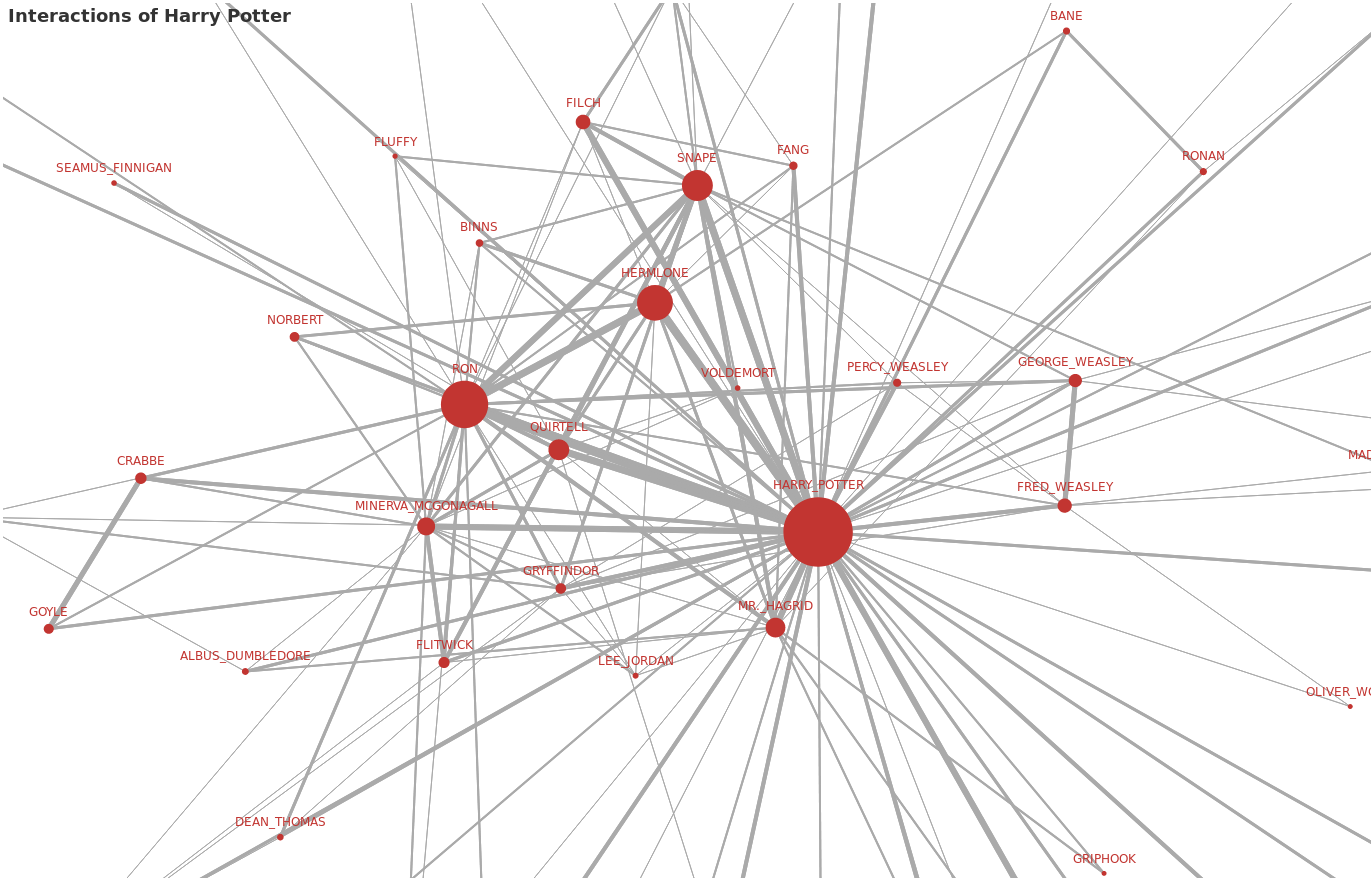
\includegraphics[width=\linewidth]{images/int_hp.png}
        \caption{Interactions in Harry Potter and the Sorcerer's Stone}
    \end{figure}
    \begin{figure}[H]
        \centering
        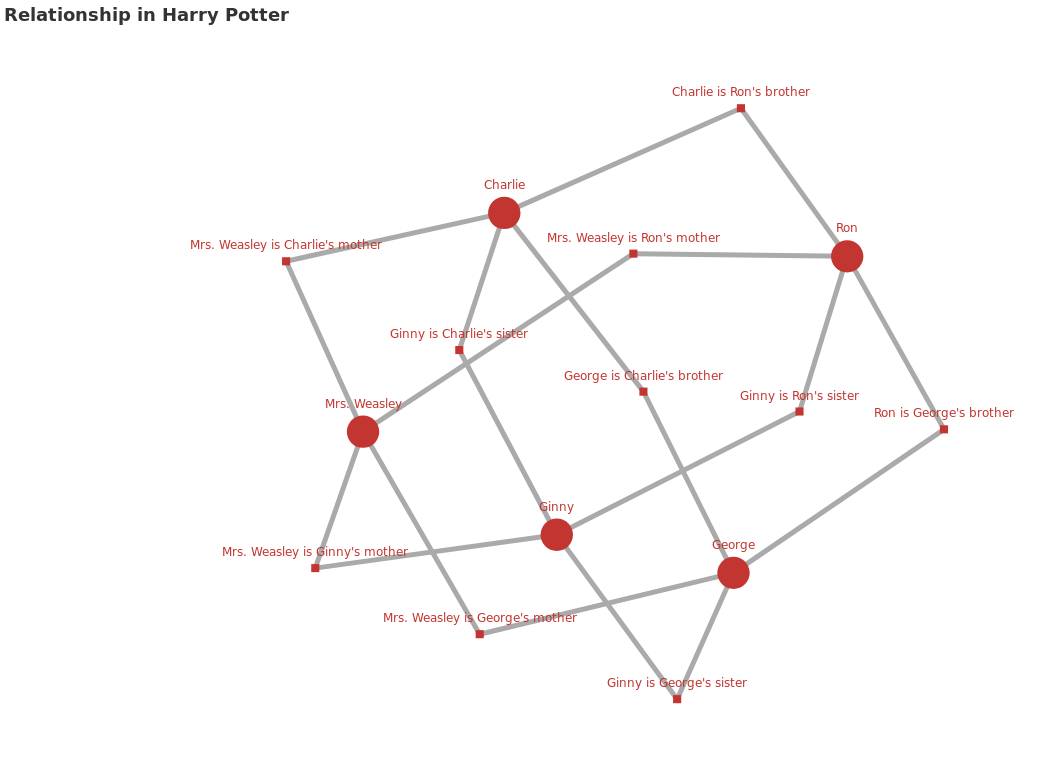
\includegraphics[width=\linewidth]{images/hp1_1.png}
        \caption{Relationships of Weasleys family}
    \end{figure}
    \begin{figure}[H]
        \centering
        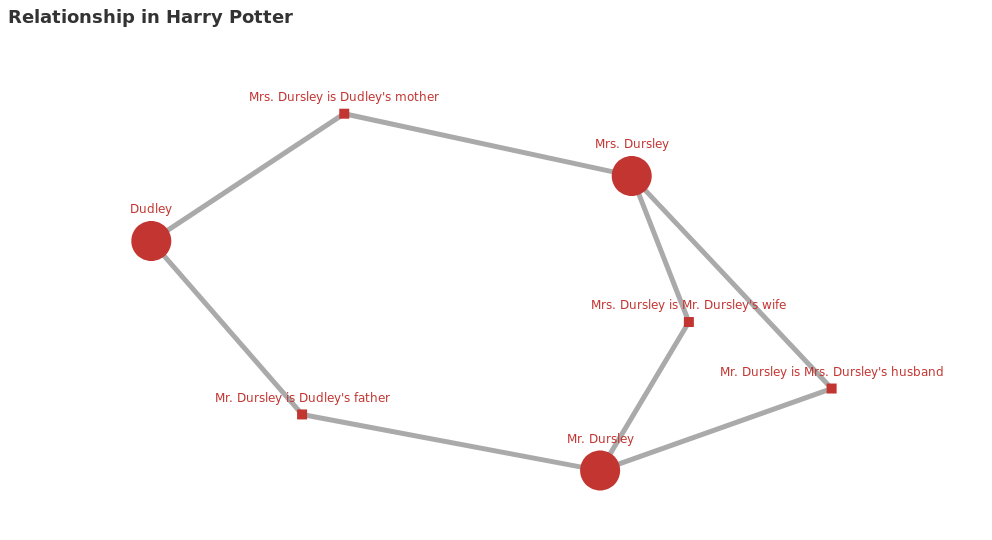
\includegraphics[width=\linewidth]{images/hp1_2.png}
        \caption{Relationships of Dursleys family}
    \end{figure}
    Since there is no available standard for us to do a quantitative evaluation, we look at the graphs we generate to do a rough evaluation. We find that for interactions part, the accuracy among main characters are close to the real situation in the novel. For the relations part, the relationship among Weasleys and Dursleys are precise. Therefore, the work we have done meets our expectation. For more detailed results, please refer to \href{github.io}{our Github}.

\subsection{Sentiment analysis}
    We visualize the sentiment matrix between roles as heatmap.
    \begin{figure}[H]
        \centering
        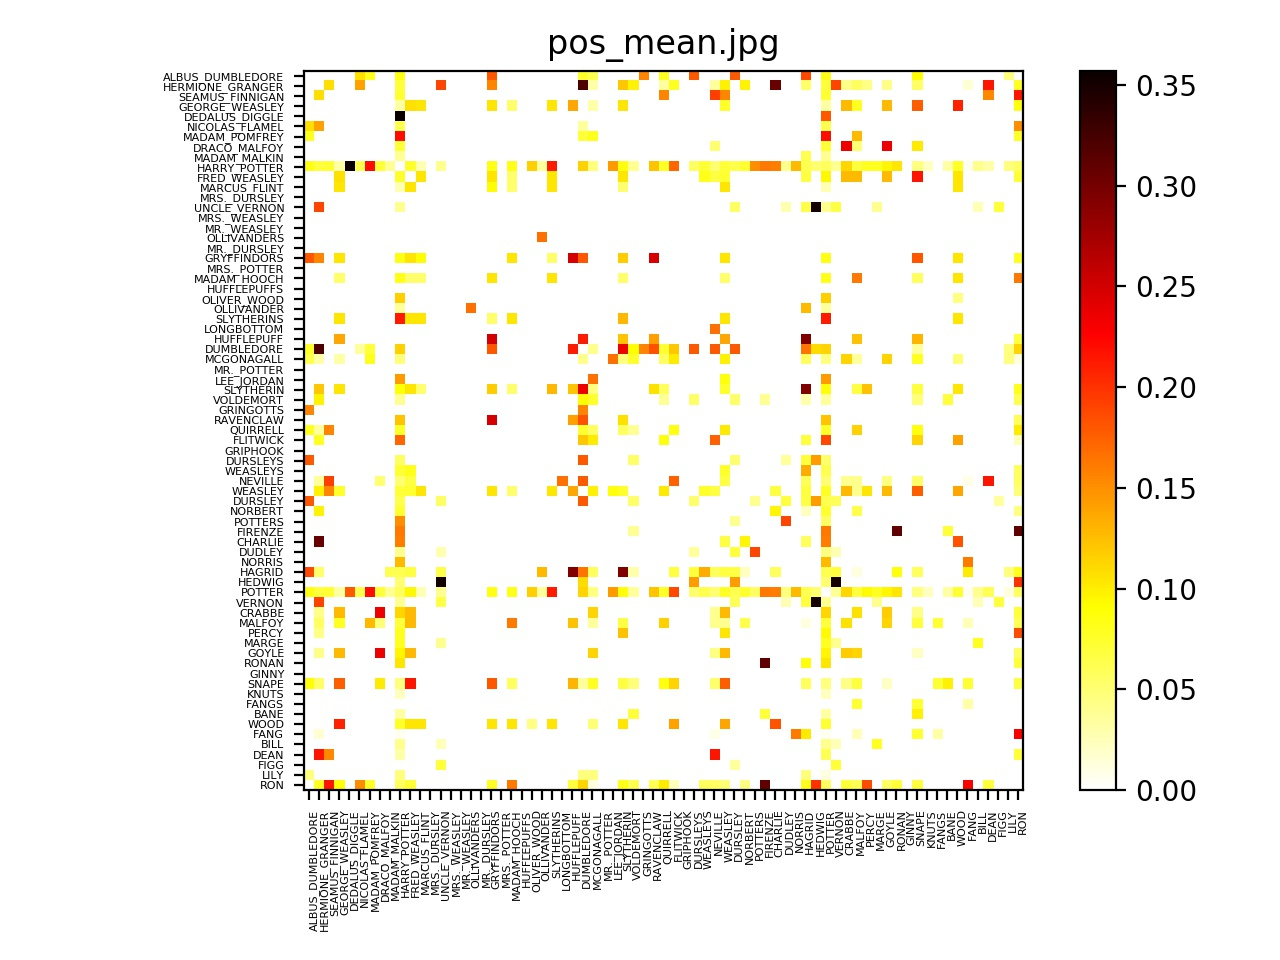
\includegraphics[width=\linewidth]{images/pos_mean.jpg}
        \caption{Mean value of positive score in Harry Potter and the Sorcerer's Stone}
    \end{figure}
    \begin{figure}[H]
        \centering
        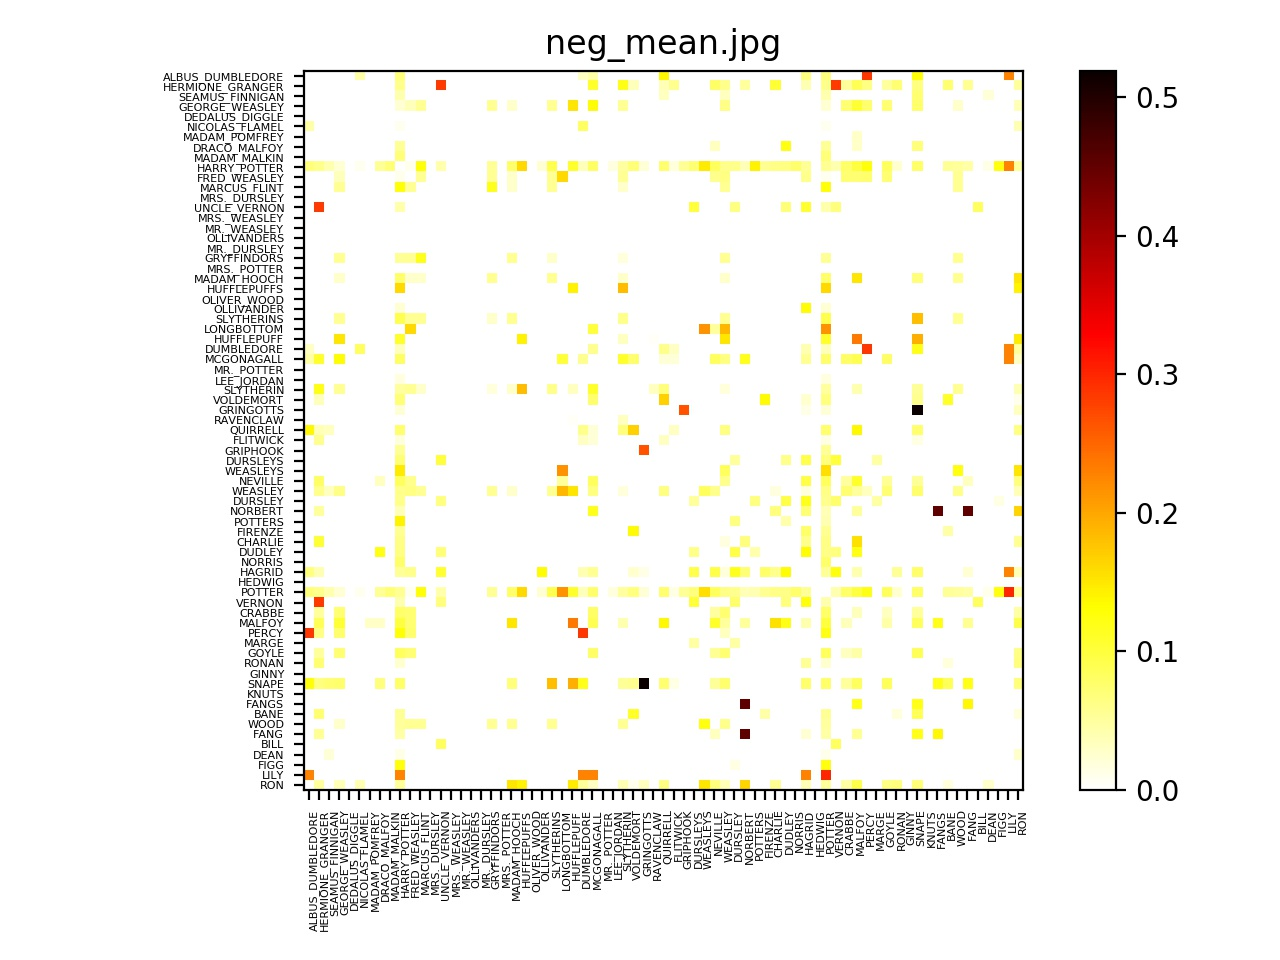
\includegraphics[width=\linewidth]{images/neg_mean.jpg}
        \caption{Mean value of negative score in Harry Potter and the Sorcerer's Stone}
    \end{figure}
    \begin{figure}[H]
        \centering
        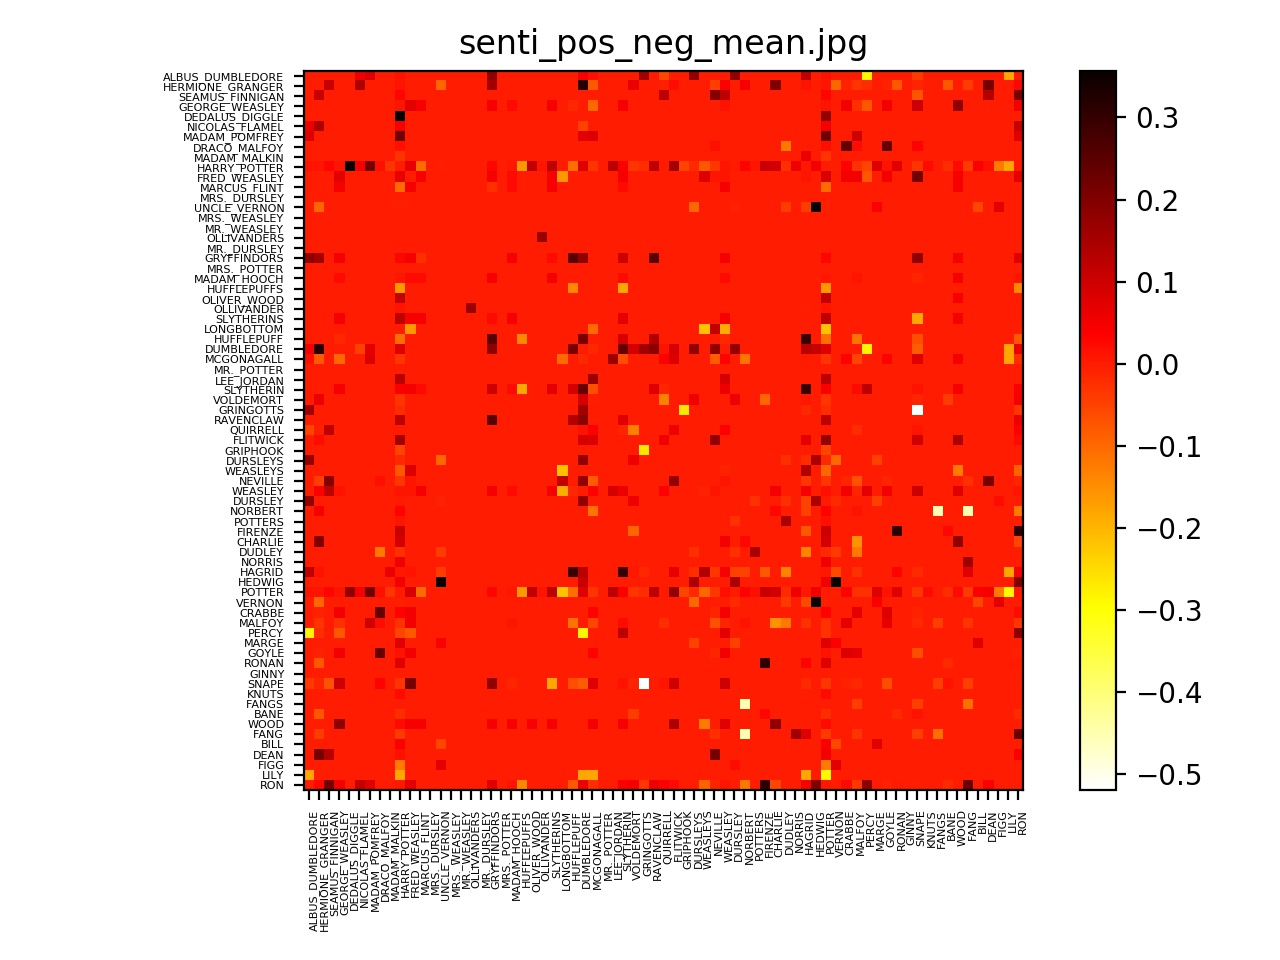
\includegraphics[width=\linewidth]{images/senti_pos_neg_mean.jpg}
        \caption{Mean value of the difference between positive and negative score in Harry Potter and the Sorcerer's Stone}
    \end{figure}

\section{Discussions} % Yunhao Li
We get good results in our test overall. However, there are still some challenges needed to be faced. For the role entity recognition, it is hard to get a perfect name dictionary. We encountered situations where the several alias of the same role cannot be merged correctly. Nicknames contribute a lot to the inaccuracy. One possible way to deal with this situation is have a dictionary of original names and nicknames. The name prefix makes it even worse. We can extract ``Mr. Weasley", but is hard to match the ``Mr. Weasley" to the one to which it truly refers (whether it refers to Ron Weasley or George Weasley). \\
For the sentiment analysis part, using polarity score is too rough and sometimes we cannot get the correct sentiment between roles. And the clustering methods doesn't work well when the Adjacency matrix is sparse. \\
For the novels like \textit{Pride and Prejudice}~\cite{pride}, the relation extraction works really well. But for the novels like \textit{Harry Potter and the Sorcerer's Stone}~\cite{harrypotter}, because there are very few explicit descriptions of the social relationships in the text, the relation extraction method doesn't work as well as the former.

\section{Conclusions} % Yunhao Li
\label{sec:length}
We develop a system that could automatically mining the data of novels, including name entity recognition and merging, coreference resolution, interaction and sentiment analysis and relation extraction. And we test it on two novels, \textit{Harry Potter and the Sorcerer's Stone}~\cite{harrypotter} and \textit{Pride and Prejudice}~\cite{pride}. The result shows that our system runs well.

\section*{Acknowledgments} % Yunhao Li

We really appreciate the work of Stanford NLP group. Their CoreNLP~\cite{corenlp} and stanfordnlp library~\cite{stanfordnlp} really help a lot. We are also grateful to the researchers and developers of Spacy~\cite{honnibal-johnson:2015:EMNLP} and NLTK~\cite{Loper02nltk:the}, and all the authors of the papers in our references. Without their great job we cannot finish our work.

% include your own bib file like this:
\bibliographystyle{acl}
\bibliography{nlp}

\end{document}